\documentclass[xetex,mathserif,serif]{beamer}
\usepackage{xeCJK}
\usepackage{amssymb,amsmath}
\usepackage{listings}
\usepackage{hyperref}
\usepackage{algorithmic,algorithm}
\usepackage{graphicx}
\usepackage{subfigure}
\usepackage{fontspec}
\usepackage{setspace}

\usecolortheme{lily}
\useoutertheme{infolines}
\useinnertheme{rectangles}
\setmainfont{Arial}
\AtBeginSection[]
{
  \begin{frame}
      \frametitle{Table of Contents}
      \tableofcontents[currentsection]
  \end{frame}
}

\begin{document}
\title[机器学习读书会报告] % (optional, only for long titles)
{读书报告}
\subtitle{第三章 \ 线性模型}
\author{刘精昌 } % (optional, for multiple authors)
\date{\today}
\subject{读书会}

\begin{frame}
\titlepage
\end{frame}

\section{线性回归模型}

\begin{frame}{引例}
  \begin{block}{工资与教育水平关系}
    考查工人工资水平与其受教育关系:
    \begin{itemize}
      \item[a] 工资水平(每小时美元数):用Y表示
      \item[b] 受教育程度(受教育年数):用X表示
      \item[c] 其他因素,如工作经验、天生素质、工作时间等其他因素
    \end{itemize}
  \end{block}
\end{frame}

\begin{frame}{引例}
    \begin{block}{工资与教育水平关系}
    \begin{itemize}
      \item[d] 观测的数据:$\left(x_i,y_i\right),i=1,\cdots,n$ (受访人数),
    \end{itemize}
    \end{block}

    \begin{center}
    \begin{tabular}{c||c c|c||c c}
      \hline
      % after \\: \hline or \cline{col1-col2} \cline{col3-col4} ...
      $i$ & $x_i$ & $y_i$ & $i$ & $x_i$ & $y_i$ \\
      \hline
      1 & 5.3 & 1.4 & 9 & 8.5 & 3.2 \\
      2 & 11.0 & 3.9 & 10 & 7.1 & 8.6 \\
      3 & 9 & 6.3 & 11 & 15 & 4 \\
      4 & 8.7 & 8.6 & 12 & 12.0 & 9.0 \\
      5 & 10 & 12 & 13 & 29 & 12 \\
      6 & 15.5 & 12 & 14 & 19.7 & 13.1 \\
      7 & 21 & 16 & 15 & 15.1 & 10 \\
      8 & 19 & 14.4 & 16 & 15.7 & 16 \\
      \hline
    \end{tabular}
    \end{center}

\end{frame}

\begin{frame}{定义}
\[ y_i = \beta_0+x_{i1}\beta_1+ \dots + x_{i,p-1}\beta_{p-1}+e_i, \ i=1,2,\dots,n\]

\[\left( {\begin{array}{*{20}{c}}
{{y_1}}\\
{{y_2}}\\
 \vdots \\
{{y_n}}
\end{array}} \right) = \left( {\begin{array}{*{20}{c}}
1&{{x_{11}}}& \cdots &{{x_{1,p - 1}}}\\
1&{{x_{11}}}& \cdots &{{x_{2,p - 1}}}\\
 \vdots & \vdots &{}& \vdots \\
1&{{x_{11}}}& \cdots &{{x_{n,p - 1}}}
\end{array}} \right)\left( {\begin{array}{*{20}{c}}
{{\beta _0}}\\
{{\beta _1}}\\
 \vdots \\
{{\beta _{p - 1}}}
\end{array}} \right) + \left( {\begin{array}{*{20}{c}}
{{e_1}}\\
{{e_2}}\\
 \vdots \\
{{e_{p - 1}}}
\end{array}} \right)\]

\[\bf{y}=\bf{X\beta}+\bf{e}\]

\end{frame}

\begin{frame}
\[ y_i = \beta_0+x_{i1}\beta_1+ \dots + x_{i,p-1}\beta_{p-1}+e_i, \ i=1,2,\dots,n\]
\begin{itemize}
  \item[(a)] 拟合值:$\mathop {{y_i}}\limits^ \wedge   = \mathop {{\beta _0}}\limits^ \wedge   + {x_{i1}}\mathop {{\beta _1}}\limits^ \wedge   \cdots  + {x_{i,p - 1}}{{\mathop \beta \limits^ \wedge}  _{p - 1}}$
  \item[(b)] 残差(residual):${\varepsilon _i} = {y_i} - {{\mathop y\limits^ \wedge}  _i} = {y_i} - \mathop {{\beta _0}}\limits^ \wedge   - {x_{i1}}\mathop {{\beta _1}}\limits^ \wedge   \cdots  + {x_{i,p - 1}}{{\mathop \beta \limits^ \wedge }_{p - 1}}$
  \item[(c)] 残差平方和(residual sum of squares \ RSS)\ $RSS = \sum\limits_{i = 1}^n {{\varepsilon _i}^2}  = \sum\limits_{i = 1}^n {{{\left( {{y_i} - \mathop {{y_i}}\limits^ \wedge  } \right)}^2}}  = {\left( {\mathop {{\rm{ }}y}\limits^ \wedge   - X\mathop \beta \limits^ \wedge  } \right)^T}\left( {\mathop {{\rm{ }}y}\limits^ \wedge   - X\mathop \beta \limits^ \wedge  } \right)$
\end{itemize}
\end{frame}

\begin{frame}{残差示意图}
\begin{figure}
  \centering
  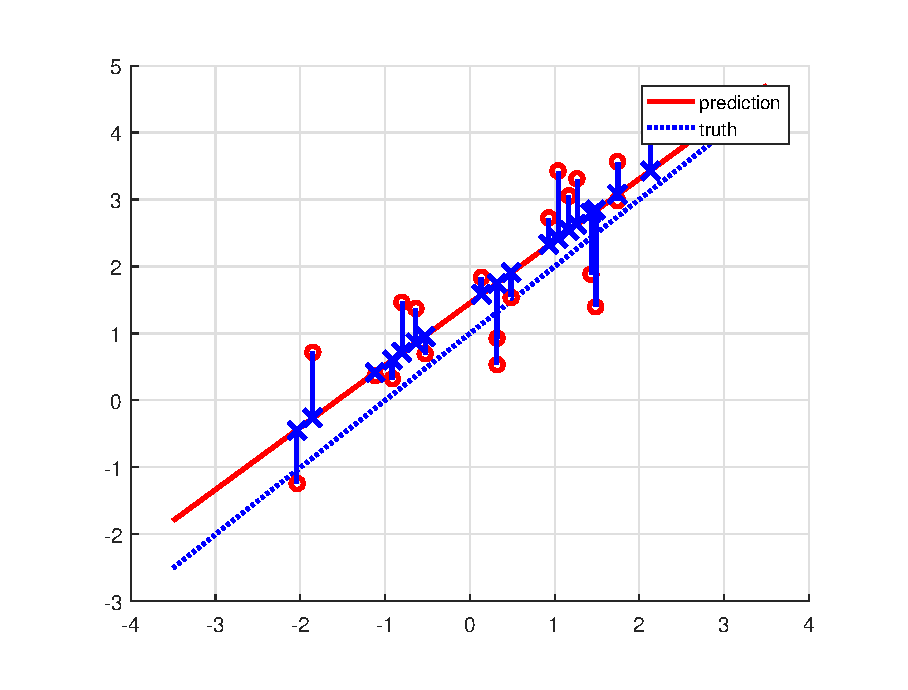
\includegraphics[width=\textwidth]{residuals.eps}
  \caption{残差示意图}\label{2}
\end{figure}

\end{frame}

\begin{frame}{参数求解}
\begin{block}{最小二乘法:RSS最小}
\begin{enumerate}
  \item $E(\mathop \beta \limits^ \wedge) = {\left( {y  - X\mathop \beta \limits^ \wedge  } \right)^T}\left( {y  - X\mathop \beta \limits^ \wedge  } \right) = y^T y - 2 y^T X \mathop \beta \limits^ \wedge + {\mathop \beta \limits^ \wedge} ^T X ^T X \mathop \beta \limits^ \wedge$
  \item $\frac{{\partial E\left( {\mathop \beta \limits^ \wedge  } \right)}}{{\partial \mathop \beta \limits^ \wedge  }} = 0$
  \item $ X^T X \mathop \beta \limits^ \wedge  = X^T y $
  \item $ \mathop \beta \limits^ \wedge = {\left( {{X^T}X} \right)^{ - 1}}{X^T}y $
\end{enumerate}
\end{block}
\end{frame}

\begin{frame}{MLE}
\begin{enumerate}
  \item ${y_i} = {\beta ^T}{x_i} + {e_i},{e_i} \sim N\left( {0,{\sigma ^2}} \right)$
  \item ${y_i} \sim N\left( {{\beta ^T}{x_i},{\sigma ^2}} \right)$
  \item $\mathop \beta \limits^ \wedge   \buildrel \Delta \over = \arg \mathop {\max }\limits_\beta  \log p\left( {D\left| \beta  \right.} \right)$

 \item $l\left( \beta  \right) \buildrel \Delta \over = \log p\left( {D\left| \beta  \right.} \right)
     = \sum\limits_{i = 1}^n {\log p\left( {{y_i}\left| \beta  \right.} \right)}
     = \sum\limits_{i = 1}^n {\log \left[ {{{\left( {\frac{1}{{2\pi {\sigma ^2}}}} \right)}^{\frac{1}{2}}}\exp \left( { - \frac{1}{{2{\sigma ^2}}}{{\left( {{y_i} - {\beta ^T}{x_i}} \right)}^2}} \right)} \right]}
      =  - \frac{1}{{2{\sigma ^2}}}RSS - \frac{N}{2}\log \left( {2\pi {\sigma ^2}} \right)$
\end{enumerate}
\end{frame}

\begin{frame}{平方和的定义}
\begin{itemize}
  \item[a、]总平方和 (Total Sum of Squares \ TSS):
  \begin{center}
    $TSS \buildrel \Delta \over = {\sum\limits_{i = 1}^n {\left( {{y_i} - \overline y } \right)} ^2},\overline y  = \frac{1}{n}\sum\limits_{i = 1}^n {{y_i}} $
  \end{center}
  \item[b、]解释平方和(Explained Sum of Squares \ ESS):
  \begin{center}
    $ESS{\rm{ }} \buildrel \Delta \over = \sum\limits_{i = 1}^n {{{\left( {{{\mathop {{\rm{ }}y}\limits^ \wedge  }_i} - \overline {\mathop {{\rm{ }}y}\limits^ \wedge  } } \right)}^2}} ,\overline {\mathop {{\rm{ }}y}\limits^ \wedge  }  = \frac{1}{n}\sum\limits_{i = 1}^n {\mathop {{y_i}}\limits^ \wedge  }  $
  \end{center}
\end{itemize}
\\
\begin{itemize}
  \item \textcolor[rgb]{1.00,0.00,0.50}{\Large{TSS = ESS + RSS}}
\end{itemize}
\end{frame}

\begin{frame}{拟合优度}
\begin{block}{判定系数的定义}
\[{R^2} = \frac{{ESS}}{{TSS}}\]
\end{block}

\begin{block}{判定系数的性质}
\begin{itemize}
  \item $0 \leq R^2 \leq 1$
  \item $R^2$ 越接近1,拟合效果越好
  \item $R^2$ 越接近0,拟合效果越差
\end{itemize}
\end{block}
\end{frame}

\begin{frame}{几何解释}
\[\mathop y\limits^ \wedge   = X\mathop \beta \limits^ \wedge   = X{\left( {{X^T}X} \right)^{ - 1}}{X^T}y\]

\begin{figure}
  \centering
  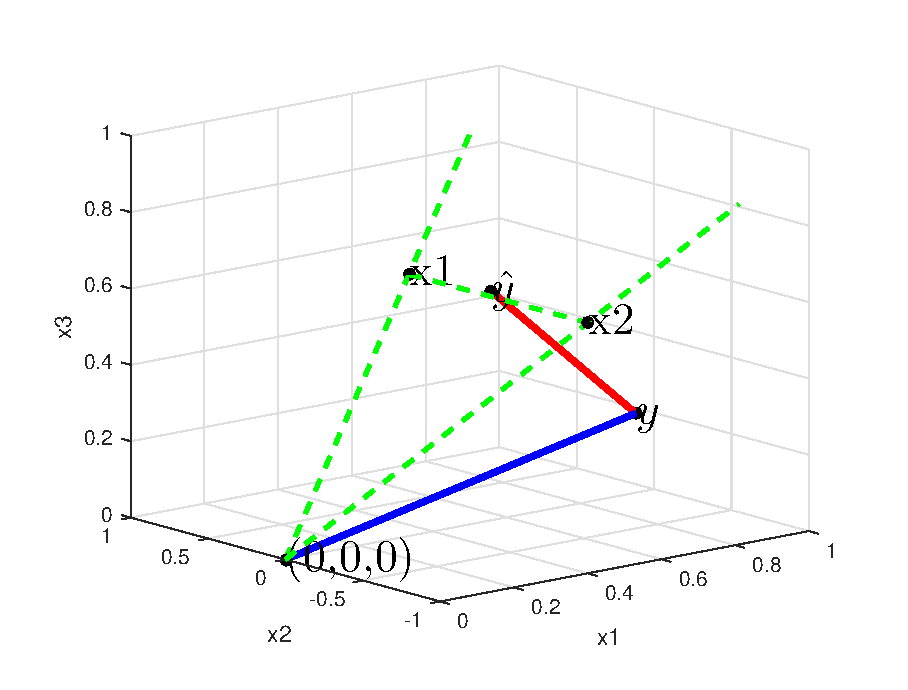
\includegraphics[width=0.7\textwidth]{projection.eps}
  \caption{$y$在$x_1 \ x_2$张成空间的投影}\label{1}
\end{figure}

\end{frame}

\begin{frame}{增加惩罚项}
\begin{block}{ridge regression}
\begin{itemize}
  \item $J\left( \beta  \right) = \frac{1}{n}RSS + \lambda \left\| \beta  \right\|_2^2$
  \item ${\mathop \beta \limits^ \wedge  _{ridge}} = \mathop {\min \arg }\limits_\beta  J\left( \beta  \right)$
  \item ${\mathop \beta \limits^ \wedge  _{ridge}} = {\left( {\lambda I + {X^T}X} \right)^{ - 1}}{X^T}y$
\end{itemize}
\end{block}

\begin{block}{LASSO}
  \[J\left( \beta  \right) = \frac{1}{n}RSS + \lambda \left\| \beta  \right\|_1\]
\end{block}
\end{frame}

\section{对数几率回归}
\begin{frame}{定义}
    \[p\left( {y\left| {x,w} \right.} \right) = Ber\left( {y\left| {sigm\left( {{w^T}x} \right)} \right.} \right) = \left\{ {\begin{array}{*{20}{l}}
    {sigm\left( {{w^T}x} \right),y = 1}\\
    {1 - sigm\left( {{w^T}x} \right),y = 0}
    \end{array}} \right.\]

    \[sigm\left( {{w^T}x} \right) = \frac{1}{{1 + {e^{{w^T}x}}}}\]
\end{frame}

\begin{frame}{sigmoid示意图}
\begin{figure}
  \centering
  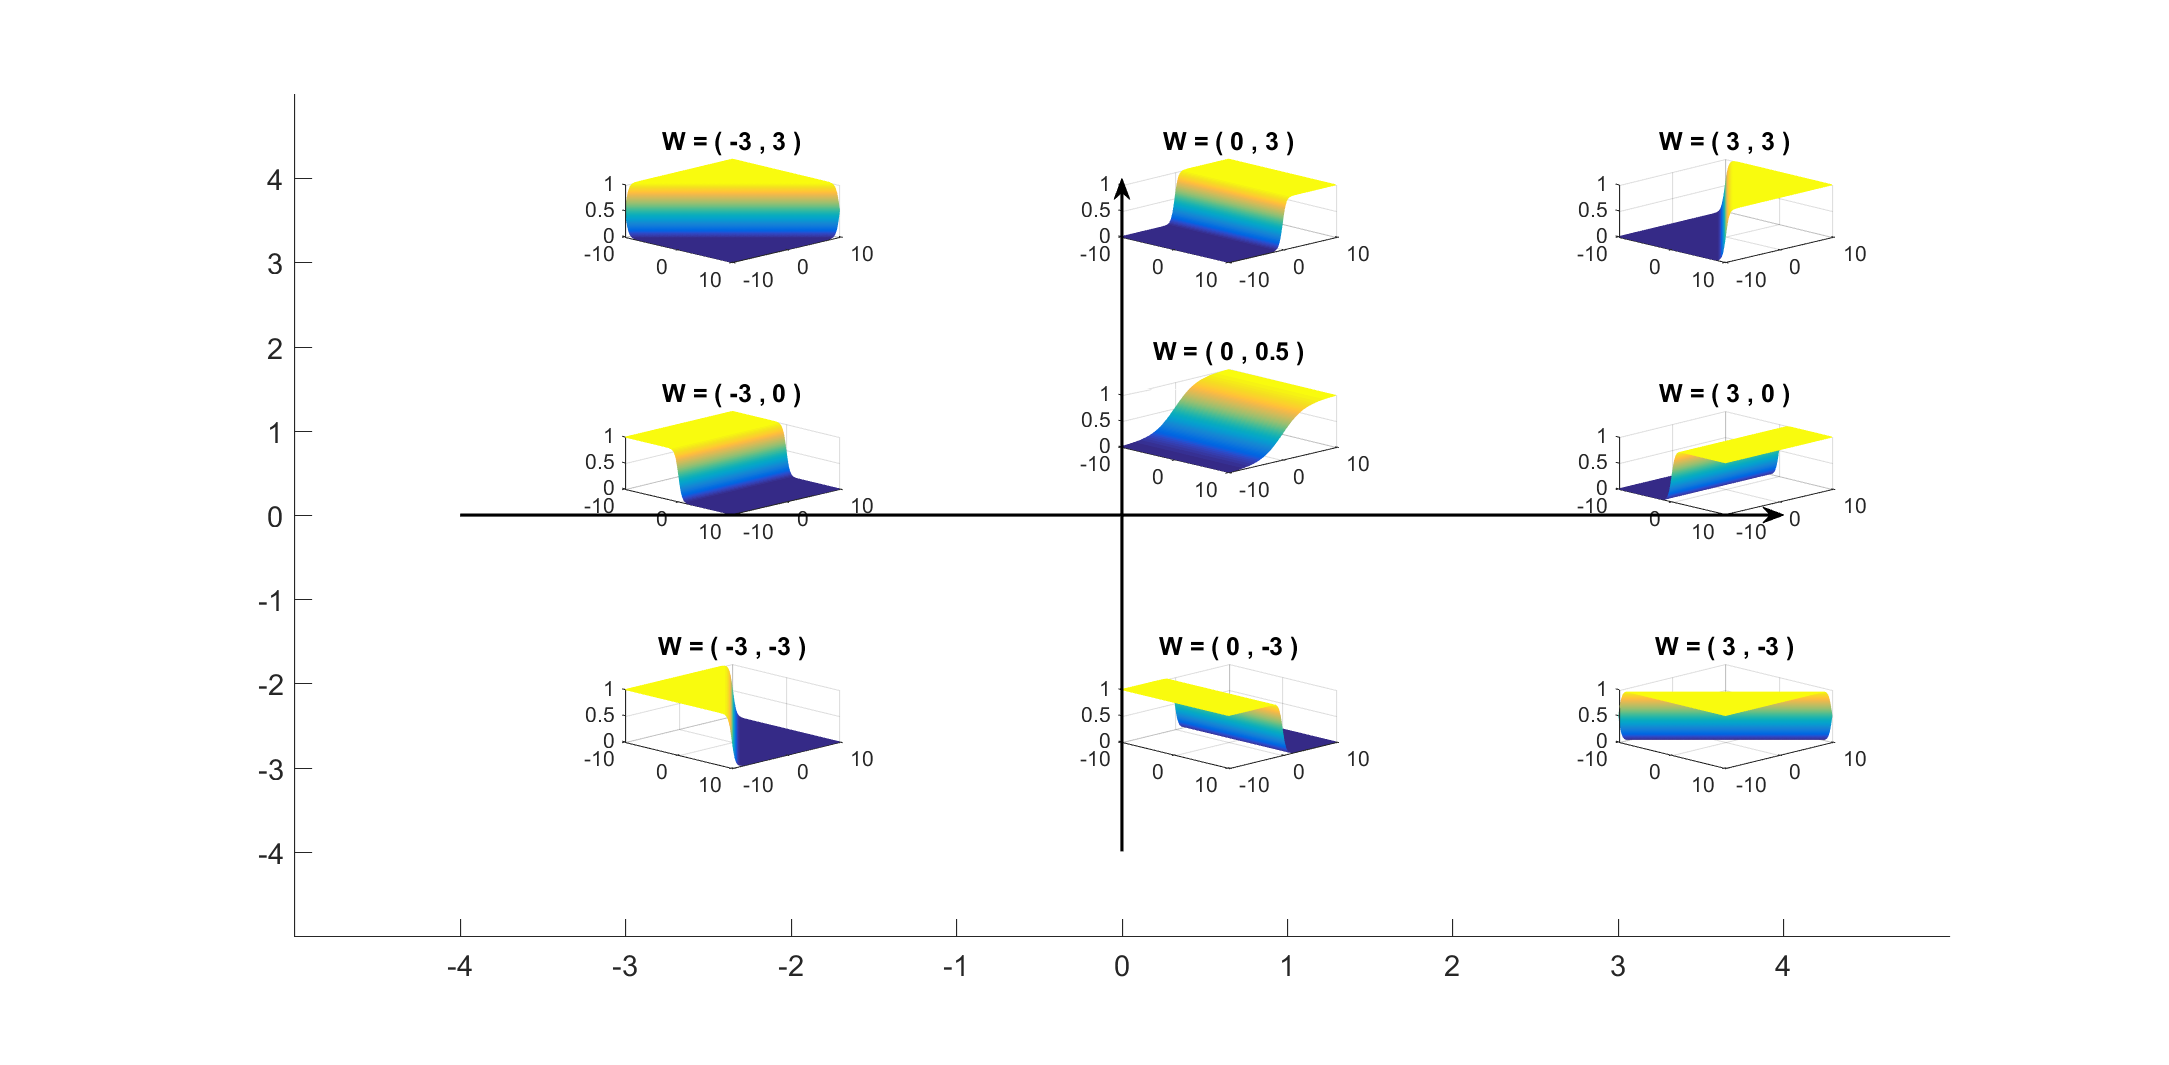
\includegraphics[width=\textwidth]{sigmoid.eps}
  \caption{sigmoid示意图}\label{3}
\end{figure}

\end{frame}

\begin{frame}{MLE}
\[{\mu _i} = sigm\left( {{w^T}{x_i}} \right) = \frac{1}{{1 + {e^{{w^T}{x_i}}}}}\]

\begin{equation*}
\begin{aligned} % requires amsmath; align* for no eq. number
    NLL\left( w \right) 
    & = - \sum\limits_{i = 1}^N {\log \left( {\mu _i^{{\rm{I}}\left( {{y_i} = 1} \right)} \times {{\left( {1 - {\mu _i}} \right)}^{{\rm{I}}\left( {{y_i} = 0} \right)}}} \right)} \\
    & =  - \sum\limits_{i = 1}^N {\left[ {{y_i}\log {\mu _i} + \left( {1 - {y_i}} \right)\log \left( {1 - {\mu _i}} \right)} \right]}
\end{aligned}
\end{equation*}
\end{frame}

\begin{frame}{MLE}
\[\frac{{\partial {\mu _i}}}{{\partial w}} =  - \frac{{{x_i}{e^{{w^T}{x_i}}}}}{{{{\left( {1 + {e^{{w^T}{x_i}}}} \right)}^2}}} =  - {x_i}{\mu _i}\left( {1 - {\mu _i}} \right)\]

\begin{equation*}
\begin{aligned} % requires amsmath; align* for no eq. number
    \frac{{\partial NLL\left( w \right)}}{{\partial w}}
    & = \sum\limits_{i = 1}^N {\frac{{\partial NLL\left( w \right)}}{{\partial {\mu _i}}}} \frac{{\partial {\mu _i}}}{{\partial w}} \\
    & = \sum\limits_{i = 1}^N {\left( {\frac{{{y_i}}}{{{\mu _i}}} - \frac{{1 - {y_i}}}{{1 - {\mu _i}}}} \right){x_i}} {\mu _i}\left( {1 - {\mu _i}} \right)\\
     & = \sum\limits_{i = 1}^N {\left( {{x_i}{y_i} - {x_i}{\mu _i}} \right)} \\
     &  = {X^T}\left( {\mu  - y} \right)
\end{aligned}
\end{equation*}
\[H = \frac{{{\partial ^2}NLL\left( w \right)}}{{\partial {w^2}}} = -{X^T}SX,S \buildrel \Delta \over = diag\left( {{\mu _i}\left( {1 - {\mu _i}} \right)} \right)\]
\end{frame}

\begin{frame}{Optimization}
    \begin{block}{Steepest descent}
    \[{\theta _{k + 1}} = {\theta _k} - {\eta _k}{g_k}\]
    \end{block}

    \begin{block}{Newton's method}
    \[{\theta _{k + 1}} = {\theta _k} - {\eta _k}H_k^{ - 1}{g_k}\]
    \end{block}
\end{frame}

\begin{frame}{softmax}
    \[\left\{ {\left( {{x^{\left( 1 \right)}},{y^{\left( 1 \right)}}} \right),\left( {{x^{\left( 2 \right)}},{y^{\left( 2 \right)}}} \right), \ldots ,\left( {{x^{\left( n \right)}},{y^{\left( n \right)}}} \right)} \right\},{y^{\left( i \right)}} \in \left\{ {1,2, \ldots ,k} \right\}\]

    \[\left[ {\begin{array}{*{20}{c}}
    {p\left( {{y^{\left( i \right)}} = 1\left| {{x^{\left( i \right)}};\theta } \right.} \right)}\\
    {p\left( {{y^{\left( i \right)}} = 2\left| {{x^{\left( i \right)}};\theta } \right.} \right)}\\
     \vdots \\
    {p\left( {{y^{\left( i \right)}} = k\left| {{x^{\left( i \right)}};\theta } \right.} \right)}
    \end{array}} \right] = \frac{1}{{\sum\limits_{j = 1}^k {{e^{w_j^T{x^{\left( i \right)}}}}} }}\left[ {\begin{array}{*{20}{c}}
    {{e^{w_1^T{x^{\left( i \right)}}}}}\\
    {{e^{w_2^T{x^{\left( i \right)}}}}}\\
     \vdots \\
    {{e^{w_k^T{x^{\left( i \right)}}}}}
    \end{array}} \right]\]
\end{frame}

\section{LDA}

\begin{frame}{LDA示意图}
\begin{figure}
  \centering
  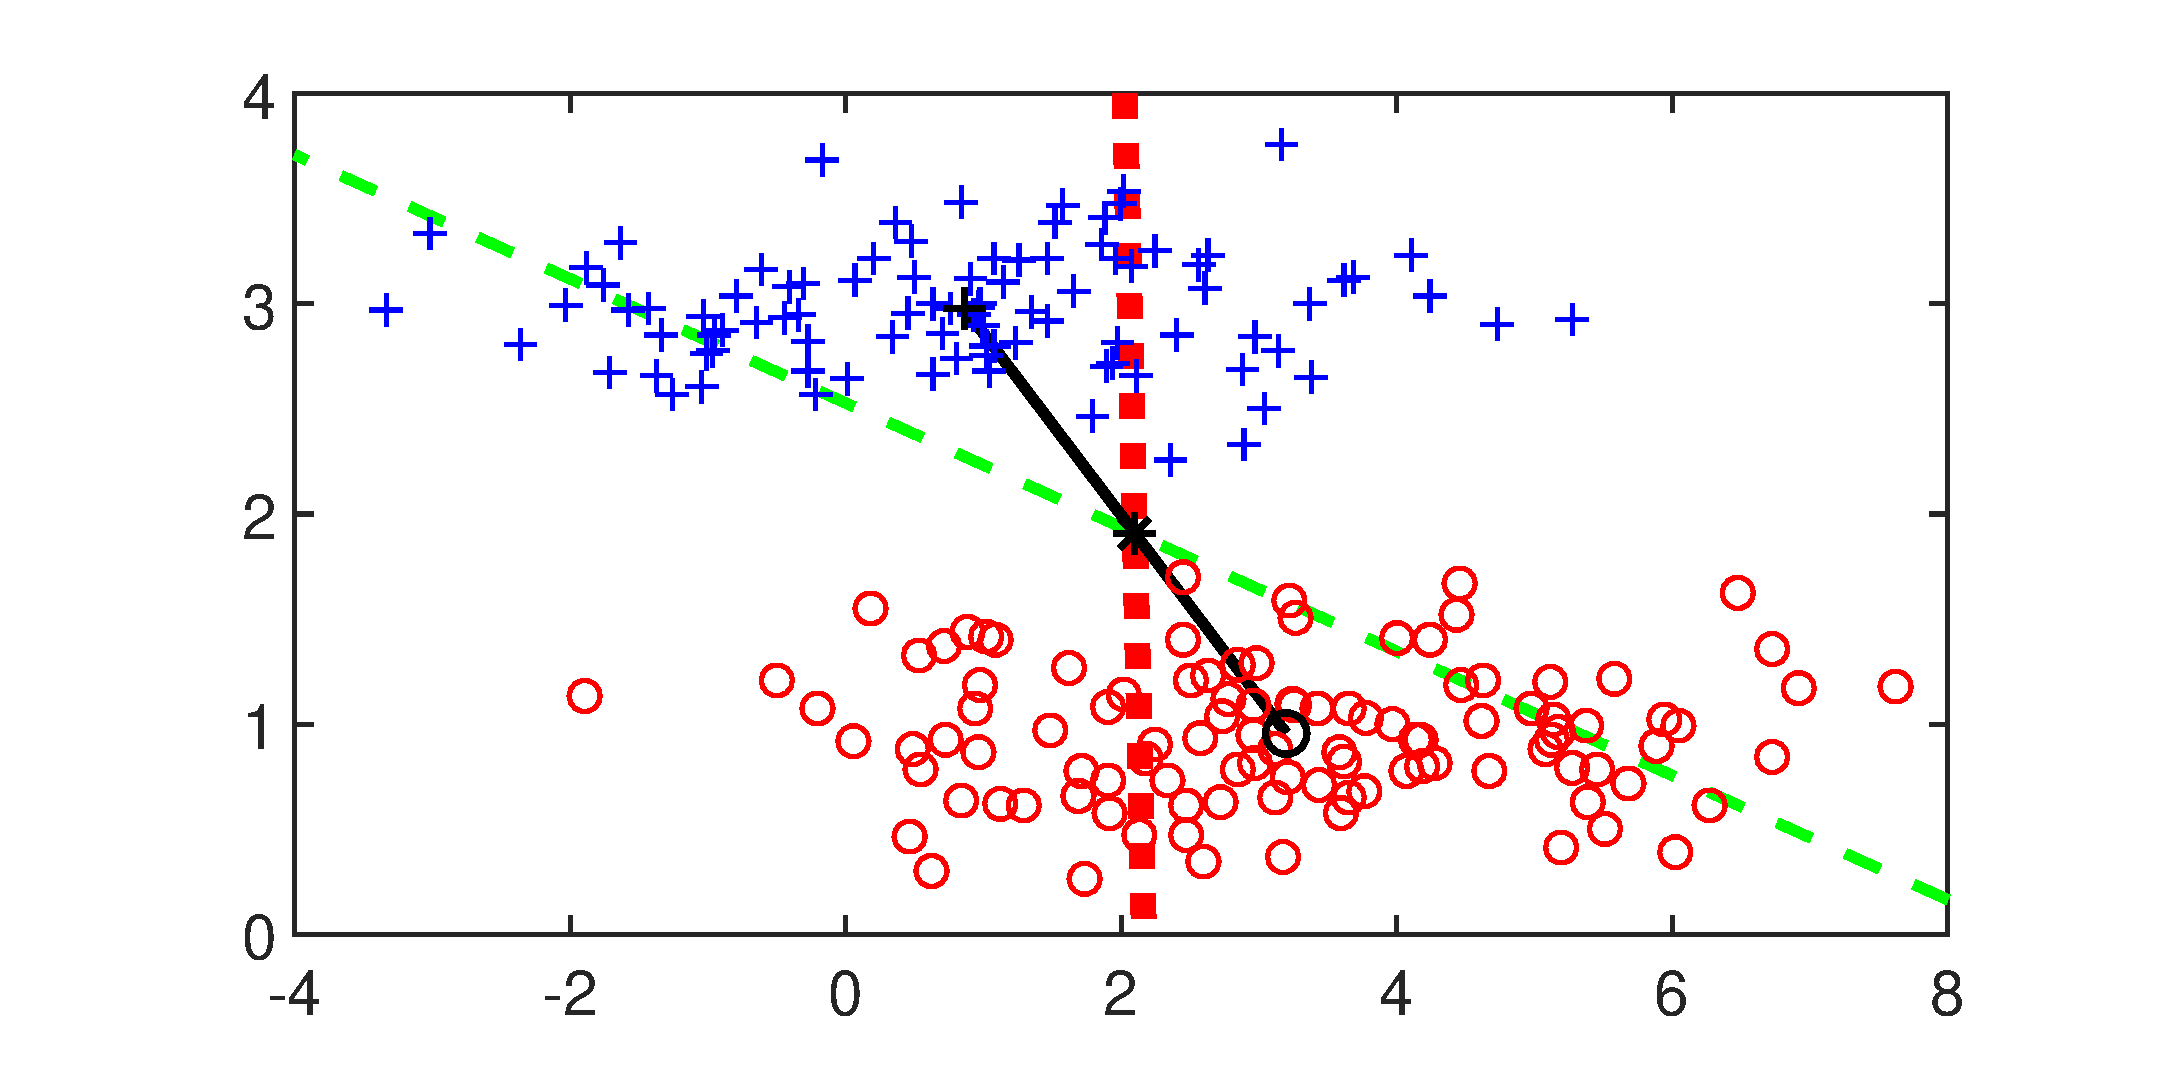
\includegraphics[width=\textwidth]{lda.eps}
  \caption{LDA示意图}\label{4}
\end{figure}

\end{frame}

\begin{frame}{LDA}
\[J\left( w \right) = \frac{{{w^T}{S_B}w}}{{{w^T}{S_W}w}}\]
\begin{itemize}
  \item between-class scatter matrix \[ S_B = (\mu_2 - \mu_1){(\mu_2 - \mu_1)}^T \]
  \item within-class scatter matrix \[{S_W} = \sum\limits_{i:{y_i} = 1} {\left( {{x_i} - {\mu _1}} \right){{\left( {{x_i} - {\mu _1}} \right)}^T}}  + \sum\limits_{i:{y_i} = 2} {\left( {{x_i} - {\mu _2}} \right){{\left( {{x_i} - {\mu _2}} \right)}^T}} \]
\end{itemize}
\end{frame}

\begin{frame}{求解}
\begin{enumerate}
  \item ${J^'}\left( w \right) = {w^T}{S_B}w - \lambda {w^T}{S_W}w,\lambda  > 0$
  \item $\frac{{d{J^'}\left( w \right)}}{{dw}} = 0$
  \item $\lambda {S_w}w = {S_B}w$
  \item ${S_B}w = \left( {{\mu _2} - {\mu _1}} \right){\left( {{\mu _2} - {\mu _1}} \right)^T}w = \left( {{\mu _2} - {\mu _1}} \right)\left( {{m_2} - {m_1}} \right)$
  \item $ w \propto S_w^{ - 1}\left( {{\mu _2} - {\mu _1}} \right)$
\end{enumerate}
\end{frame}

\begin{frame}
\begin{center}
  \Large {Q \& A}
\end{center}
\end{frame}

\end{document} 